\newcommand{\pyred}{\textsc{PyReduce}}
\newcommand{\met}{\ac{METIS}}
\newcommand{\mir}{\ac{MIR}}
\newcommand{\lss}{\ac{LSS}}
\newcommand{\elt}{\ac{ELT}}
\newcommand{\scope}{\textsc{ScopeSim}}

% The goal of this calibration step is to create rectified 2D orders with the spatial coordinate along the slit and the calibrated wavelength coordinate along the dispersion direction. This can be achieved in three steps:

The \mir~range is dominated by thermal and line emission in the Earth's atmosphere. These emission lines can be used to determine both the curvature/tilt-distortion of the LSS spectrograph and subsequently the wavelength calibration. We adapt the \pyred~package \cite{pis21} employing state-of-the-art functions for optimal extraction of echelle spectra.  The package works successfully on several ESO instruments and has been adopted for the CRIRES+ pipeline. In the following sections we assess its functionality on simulated \met~ spectroscopic data.


\subsubsection{Implementing METIS in \pyred}\label{sec:pyred_mic}
% \todo[inline]{TODO-NS: to be edited}
\pyred~\cite{pis21} is an  open source Python implementation\footnote{\url{https://github.com/AWehrhahn/PyReduce}} (with some C components)  of the IDL-based REDUCE pipeline \cite{pis02}.  The package supports data reduction of several echelle spectrographs, e.g. CRIRES+,  HARPS, and can be optimized to work on any instrument, also on a  long slit spectrograph as in the case of \met. In order to adapt \pyred~to work on simulated \met~\lss~data, we created a custom instrument class  and defined all the needed parameters to run \pyred~within a single script (Method~1\footnote{\url{https://pyreduce-astro.readthedocs.io/en/latest/instruments.html}}). This provided a quick way to finding the needed settings to  run the package successfully on \met~data before a complete implementation is done following Method~2. The full implementation requires several configuration files: 
\begin{itemize}
\item Custom instrument class (\texttt{metis.py}) serving several functions such as loading a json file (\texttt{load\_info}) with FITS header information, finding  and sorting files (\texttt{sort\_files}) for the different reduction steps, modifying fits header information (\texttt{add\_header\_info}), finding the wavelength calibration guess file (\texttt{get\_wavecal\_filename}) etc.
\item Header keyword map (\texttt{metis.json})
\item \pyred~runtime configuration file (\texttt{settings\_metis.json}) 
\item Wavelength calibration initial guess  file (e.g. \texttt{metis\_lss\_m\_2D.npz}) containing a numpy recarray called \texttt{cs\_lines} which includes information on the detector positions of the wavelength calibration lines.
 % and their respective echelle orders. 
 More details in Sect.~\ref{sec:critalg_wavecal}
\item \pyred~runtime script (\texttt{metis\_example.py}), in which the user defines where the data are located, which \met~\lss~mode to use ($L$, $M$, or $N$-band), \pyred~steps to run, and where they could change any parameter pertaining to \pyred~steps before inserting them into the file \texttt{settings\_metis.json}.
\end{itemize}

Placing the above files in their respective \pyred~folders enables \pyred~to run \met~\scope~simulated files as any other instrument. \pyred~ performs many functions when reducing spectroscopic data  including basic data reduction like bias determination, flatfielding, continuum fitting. Here we investigate mainly the steps relevant to the mentioned critical algorithms: \texttt{"curvature", and "wavecal"}.
%-----------
\paragraph{Simulated input `raw' data}
To demonstrate the feasibility of adopting \pyred~algorithms to \met~purposes we use data simulated with \scope~for all three \lss~modes ($L$, $M$, or $N$-band) for the $8000~\mathrm{mas} \times 19~\mathrm{mas}$ slit (see Fig.~\ref{fig:lmn_layout}). 
% \todo Details on the simulated data and the input files and settings used to generate them are listed in the DRLVT \cite{drlvt}. 
Then header keywords of the simulated data were added/modified to enable \pyred~to sort the individual files according to \texttt{metis.json}. Here we list the files - listed here for the case of $L$-band but similarly to $M$ and $N$-bands - that are used to operate \pyred, which can be downloaded from\footnote{\url{https://www.dropbox.com/sh/h1dz80vsw4lwoel/AAAqJD_FGDGC-t12wgnPXVR8a?dl=0}}: 
\begin{itemize}
   \item \texttt{lss\_l\_thermal.fits}: spectroscopic flat field (Fig.~\ref{fig:ff})
   \item \texttt{lss\_l\_pinholes.fits}: pinhole frame with the flat field (Fig.~\ref{fig:pinh})
   \item \texttt{lss\_l\_sky.fits}: sky emission line spectrum covering the full slit (Fig.~\ref{fig:sky})
   \item \texttt{lss\_l\_star.fits}: star spectrum ("science" target) (Fig.~\ref{fig:star})
\end{itemize}

\begin{figure}[!ht]
  \centering
  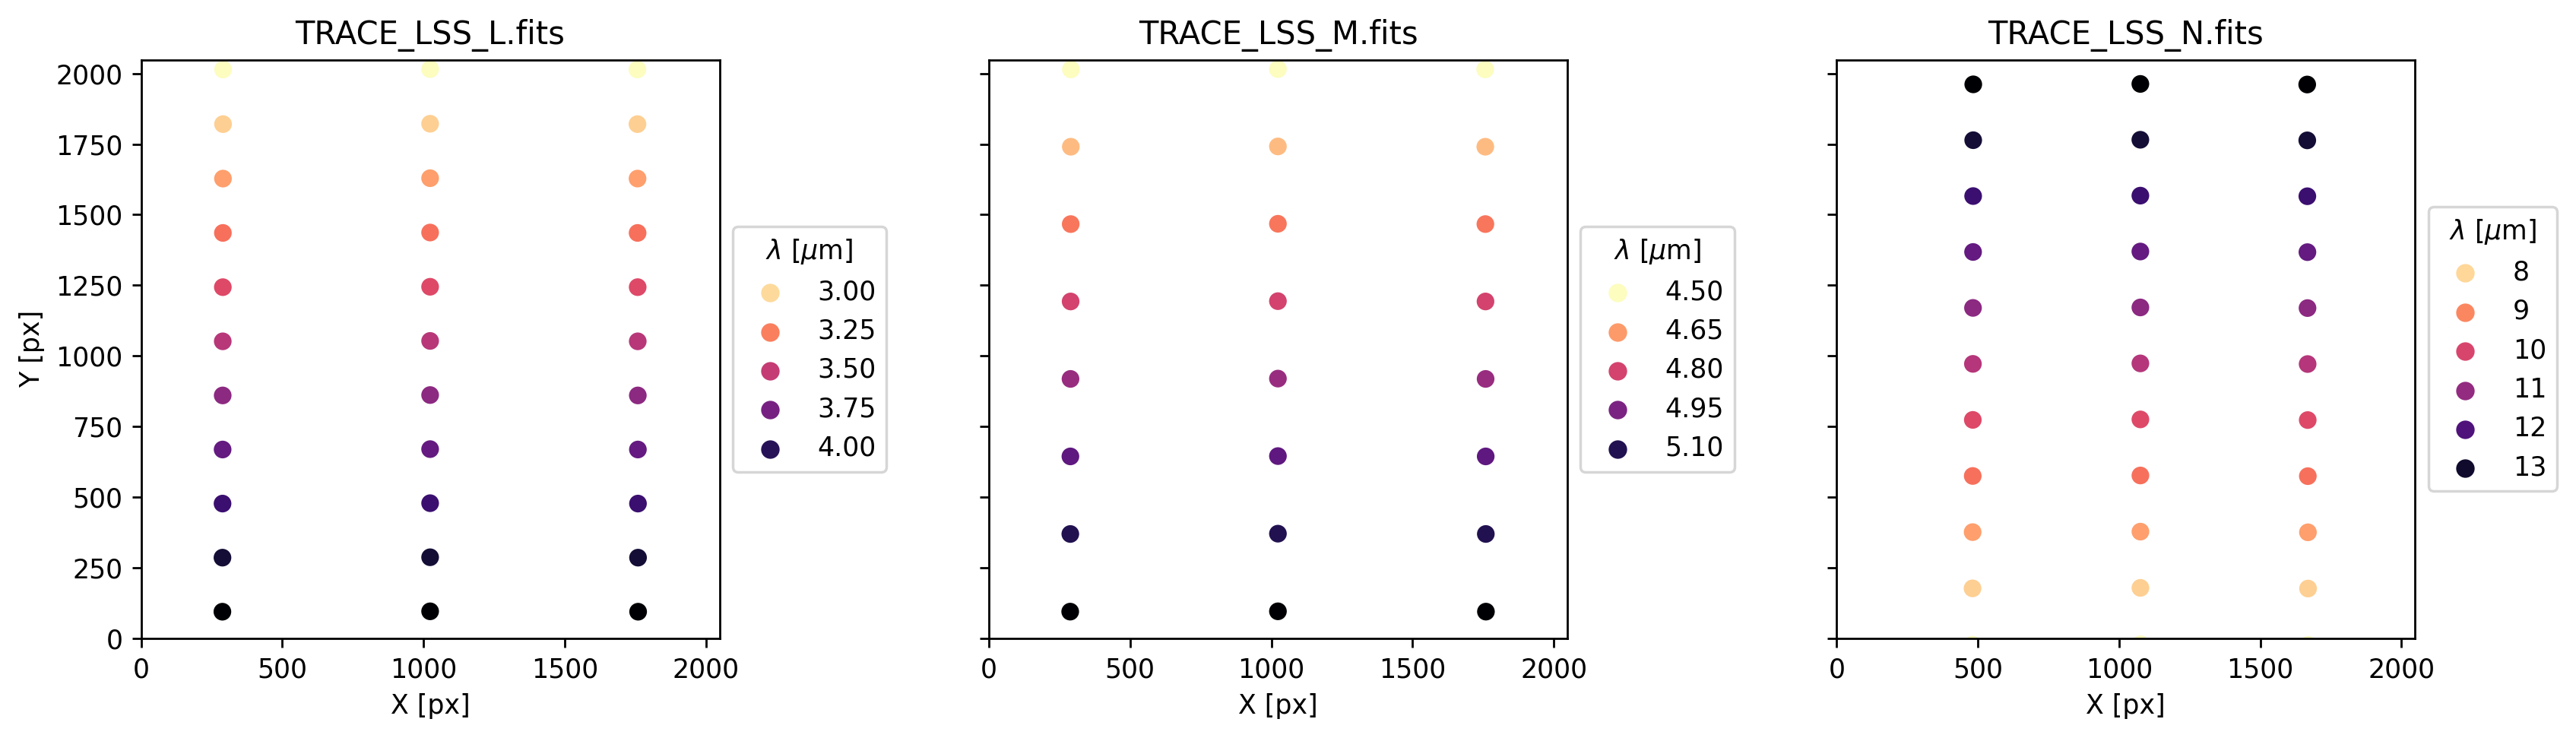
\includegraphics[width=\textwidth]{figures/LSS_CrtAlg_files/METIS_LSS_SpectralLayout_px.png}
  \caption{\textbf{Spectral layout of the METIS LSS mode of all three supported bands}: The spectral layout is shown here for all three \lss~bands as taken from the corresponding trace files - after transforming from mm to px coordinates- from the \met~IRDB for a slit length of 8 arcsec.}
  % \caption{\textbf{Spectral layout of the METIS LSS mode of all three supported bands}: The spectral layout is shown here for all three \met~\lss~bands where sky emission lines fall on them. }

  \label{fig:lmn_layout}
\end{figure}

\begin{figure}[!ht]
\centering
  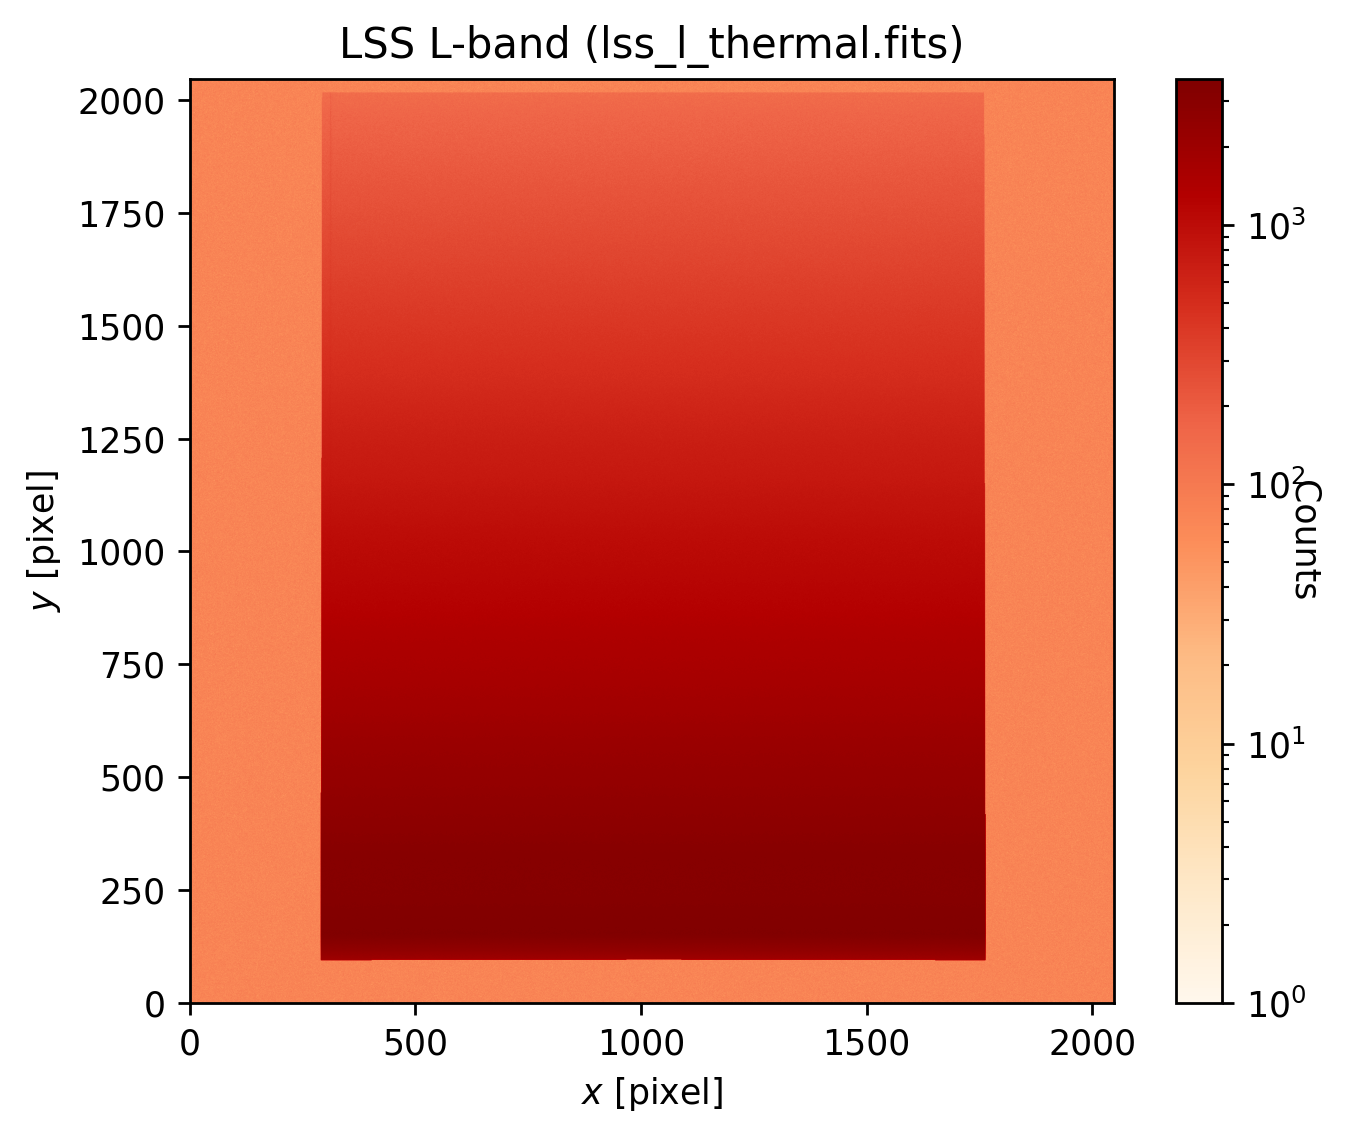
\includegraphics[height=4cm,keepaspectratio]{figures/LSS_CrtAlg_files/lss_l_thermal.fits.png}
  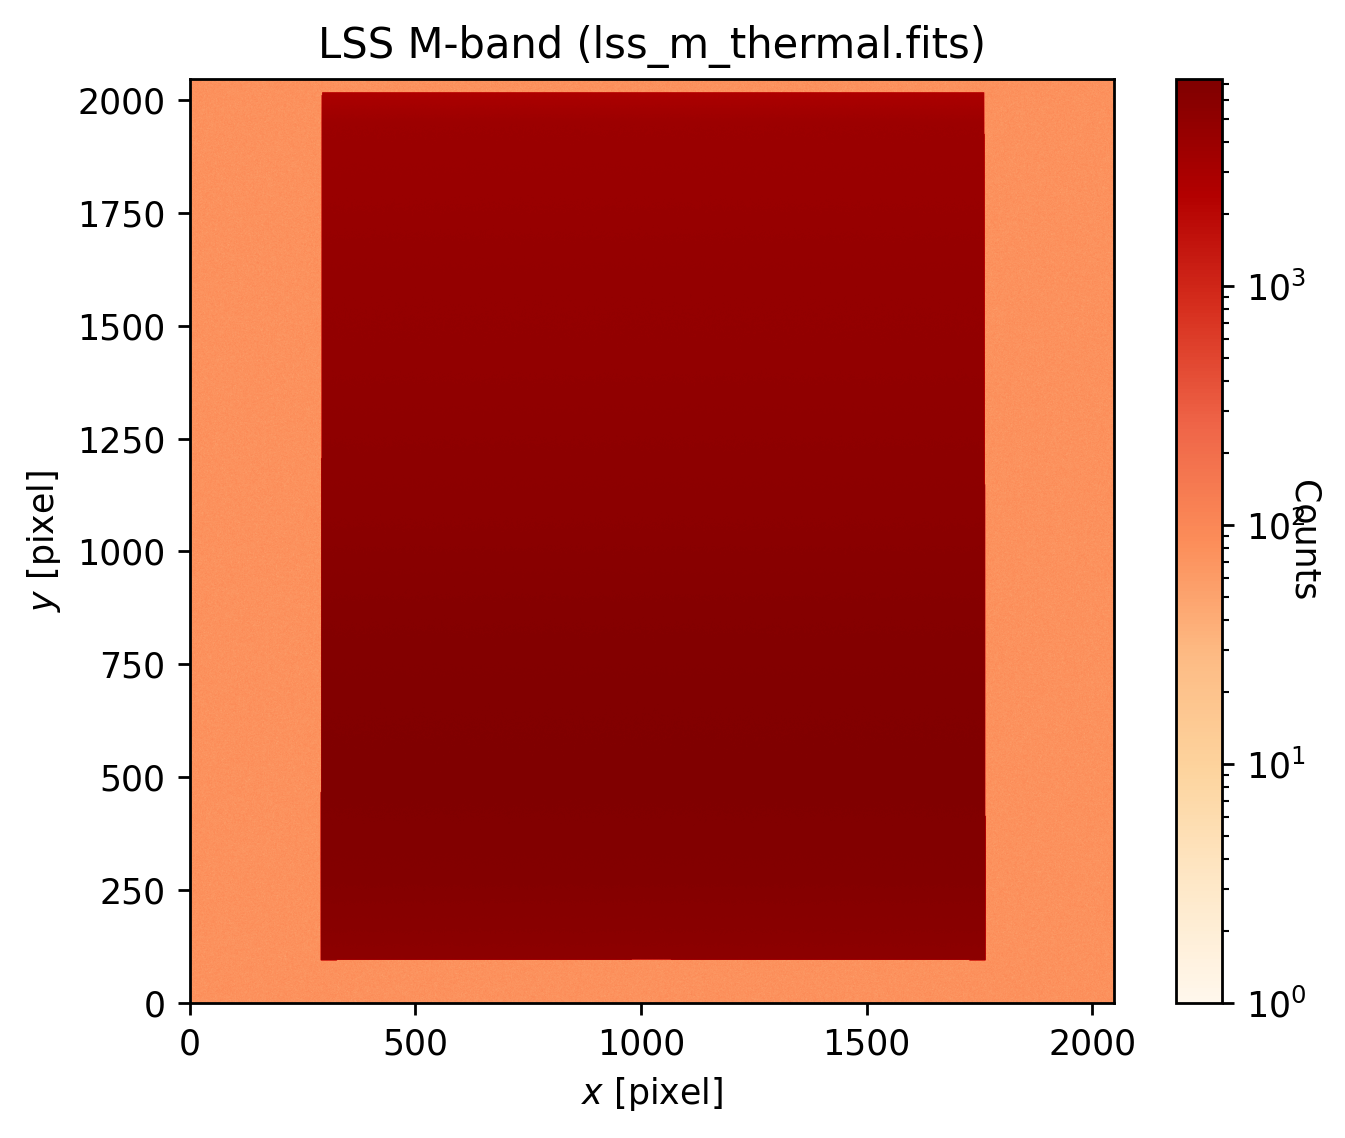
\includegraphics[height=4cm,keepaspectratio]{figures/LSS_CrtAlg_files/lss_m_thermal.fits.png}
  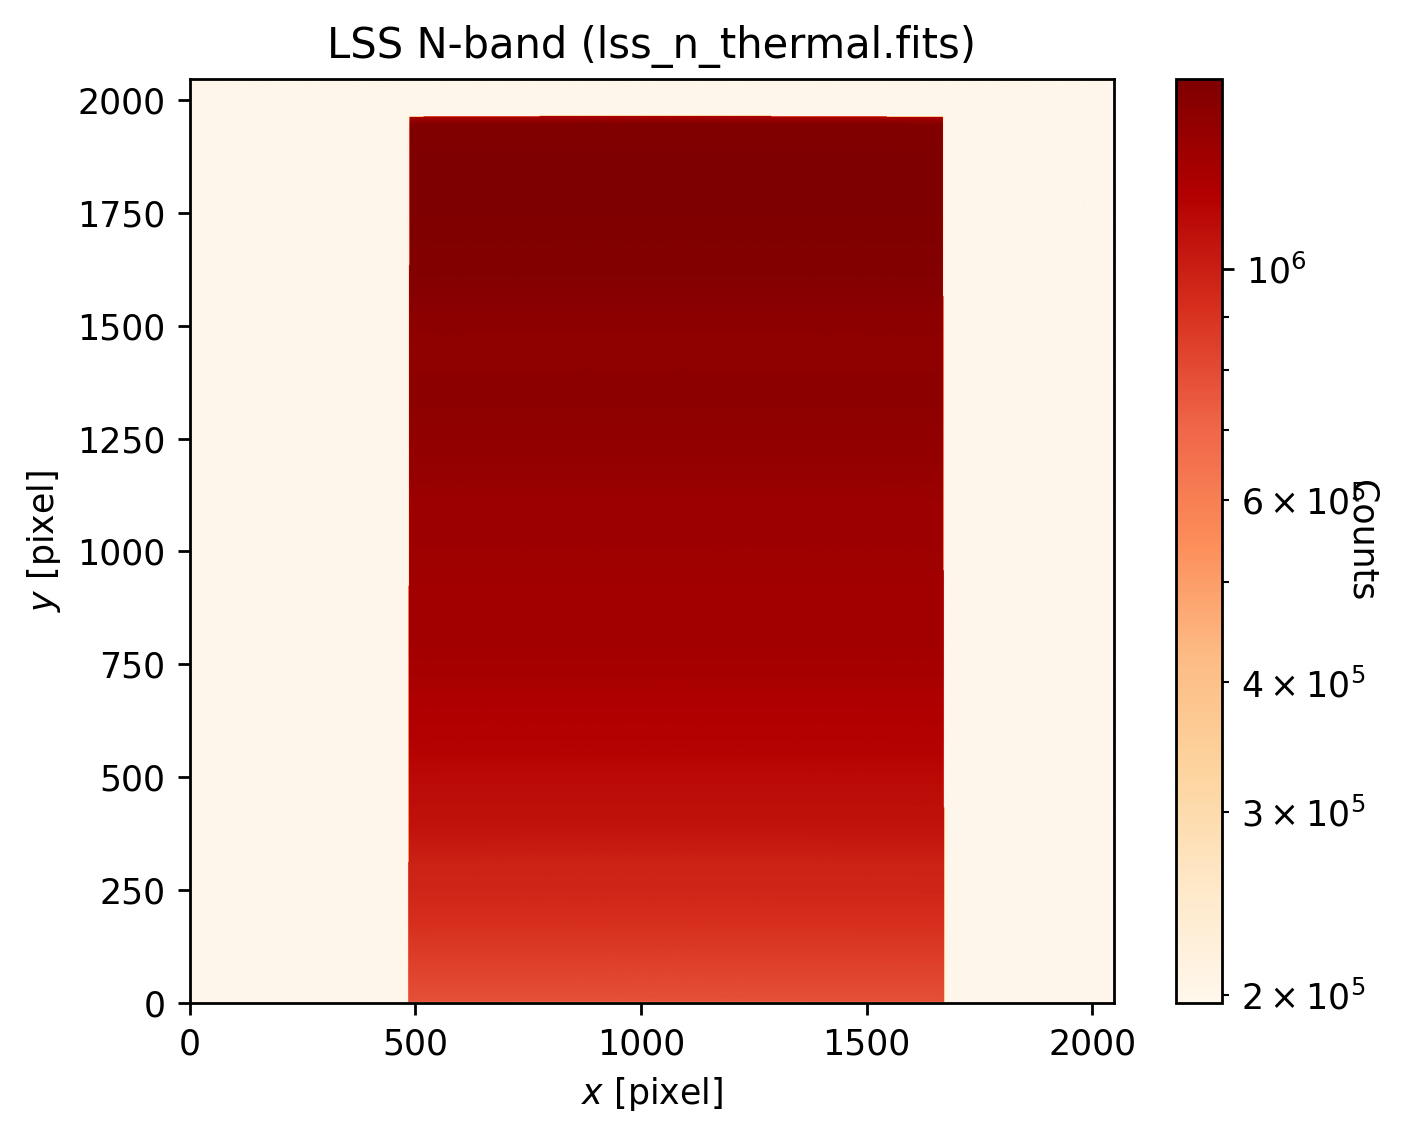
\includegraphics[height=4cm,keepaspectratio]{figures/LSS_CrtAlg_files/lss_n_thermal.fits.png}
  \caption{Long-slit spectroscopic flat field frames for \lss~$L$-, $M$-, and $N$-bands.} 
  \label{fig:ff}
\end{figure}

\begin{figure}[!ht]
\centering
  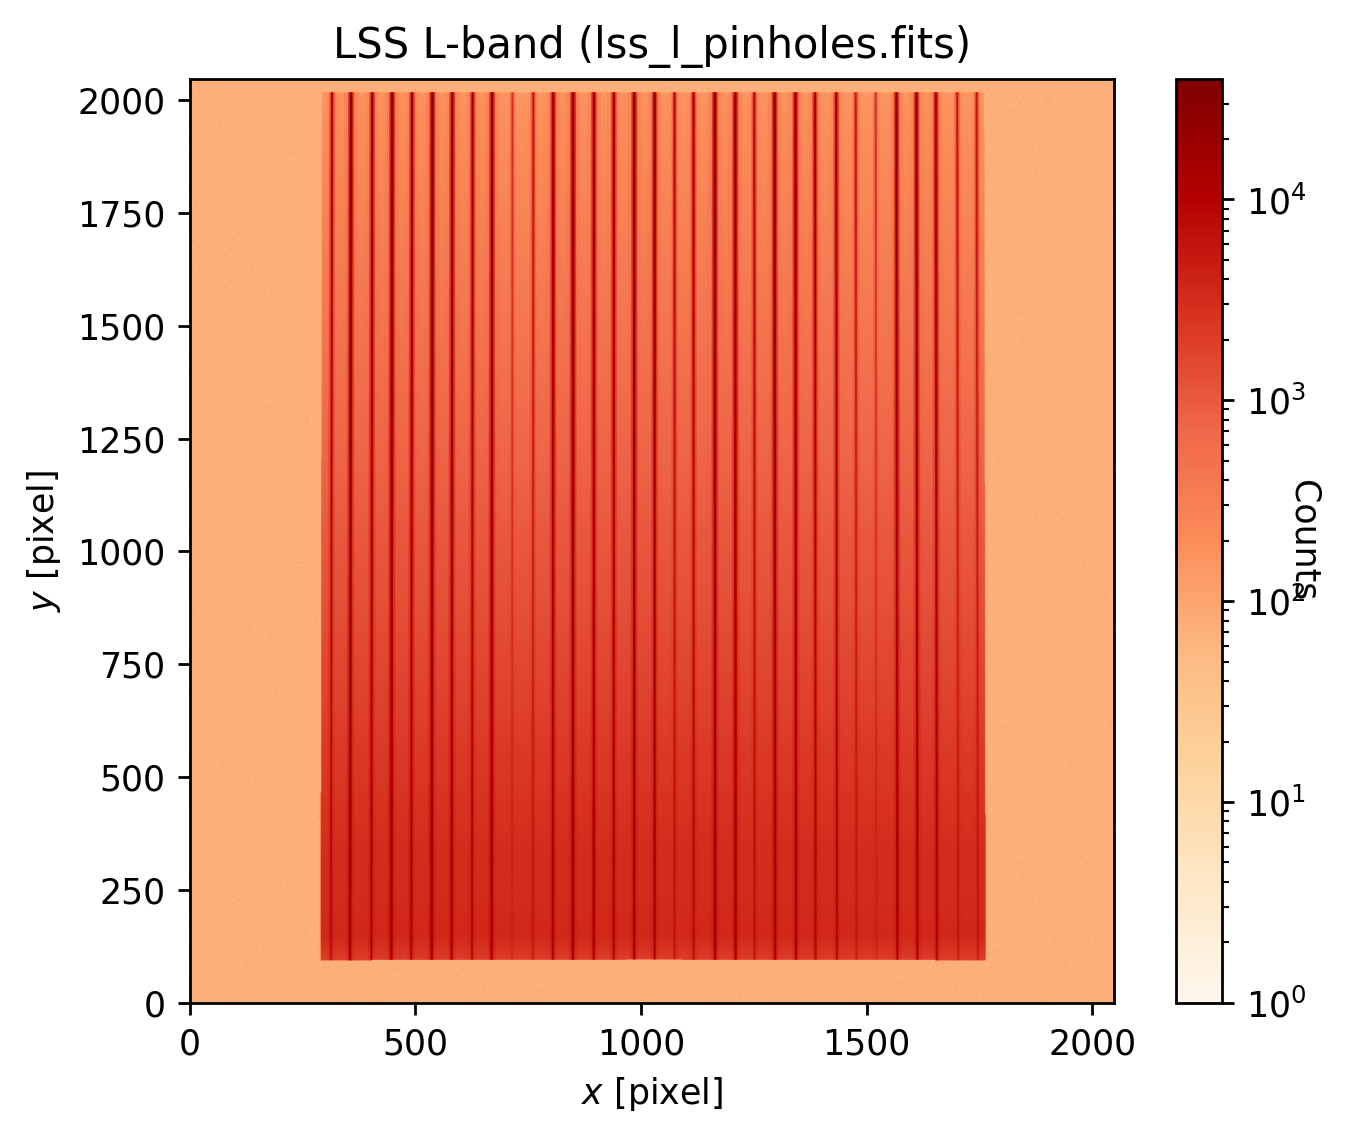
\includegraphics[height=4cm,keepaspectratio]{figures/LSS_CrtAlg_files/lss_l_pinholes.fits.png}
  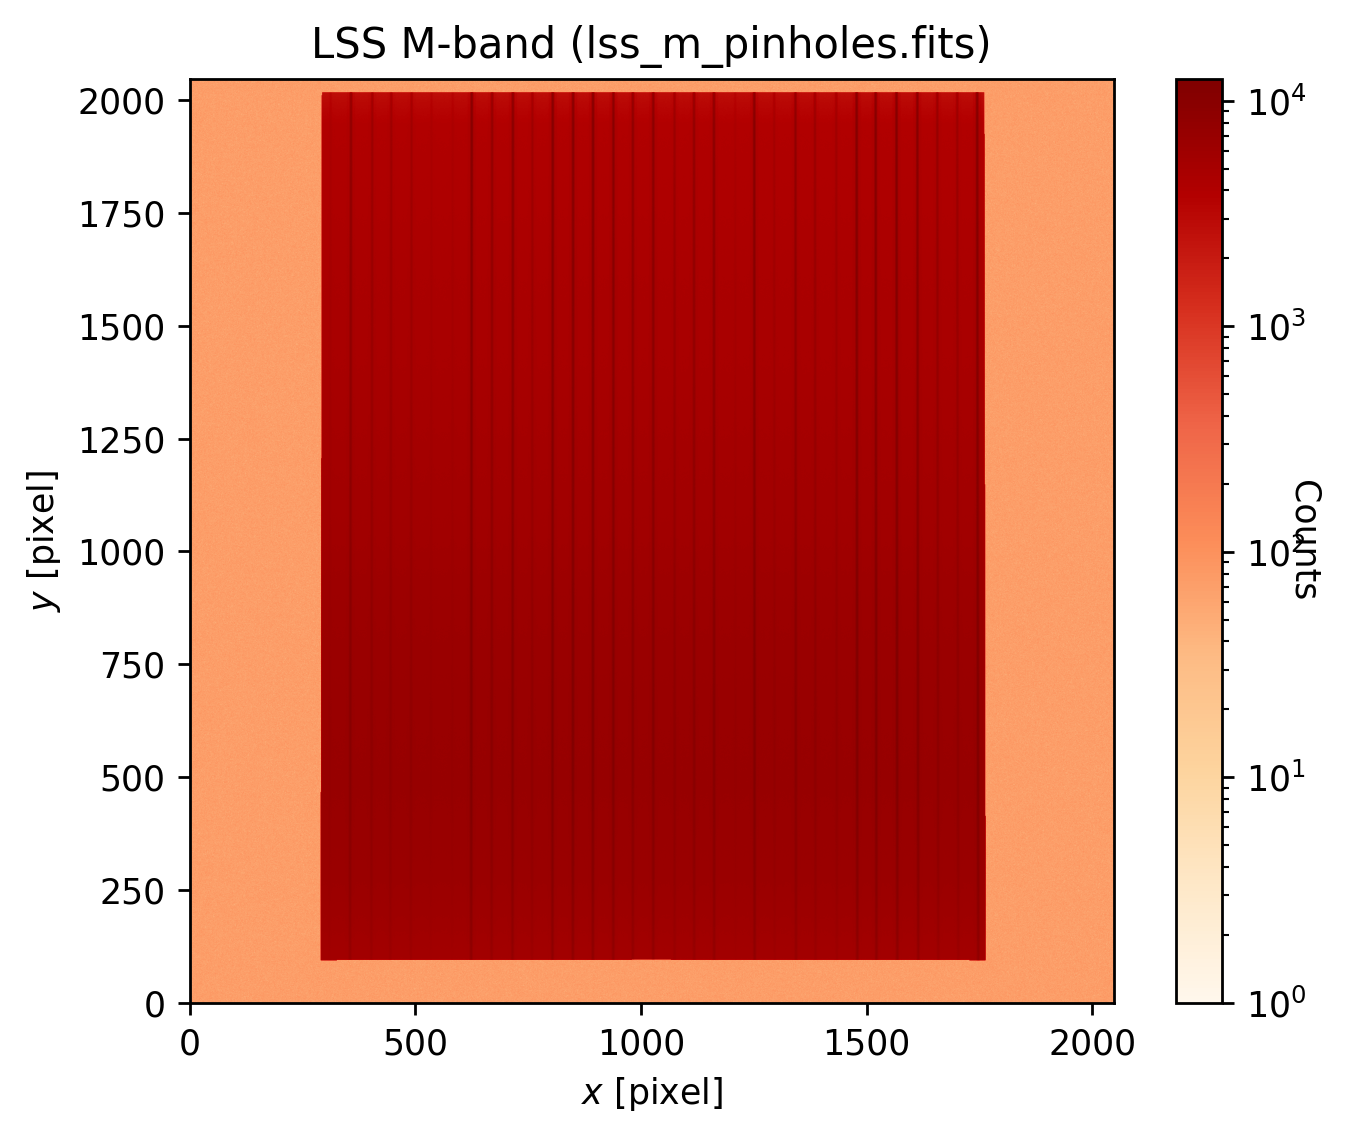
\includegraphics[height=4cm,keepaspectratio]{figures/LSS_CrtAlg_files/lss_m_pinholes.fits.png}
  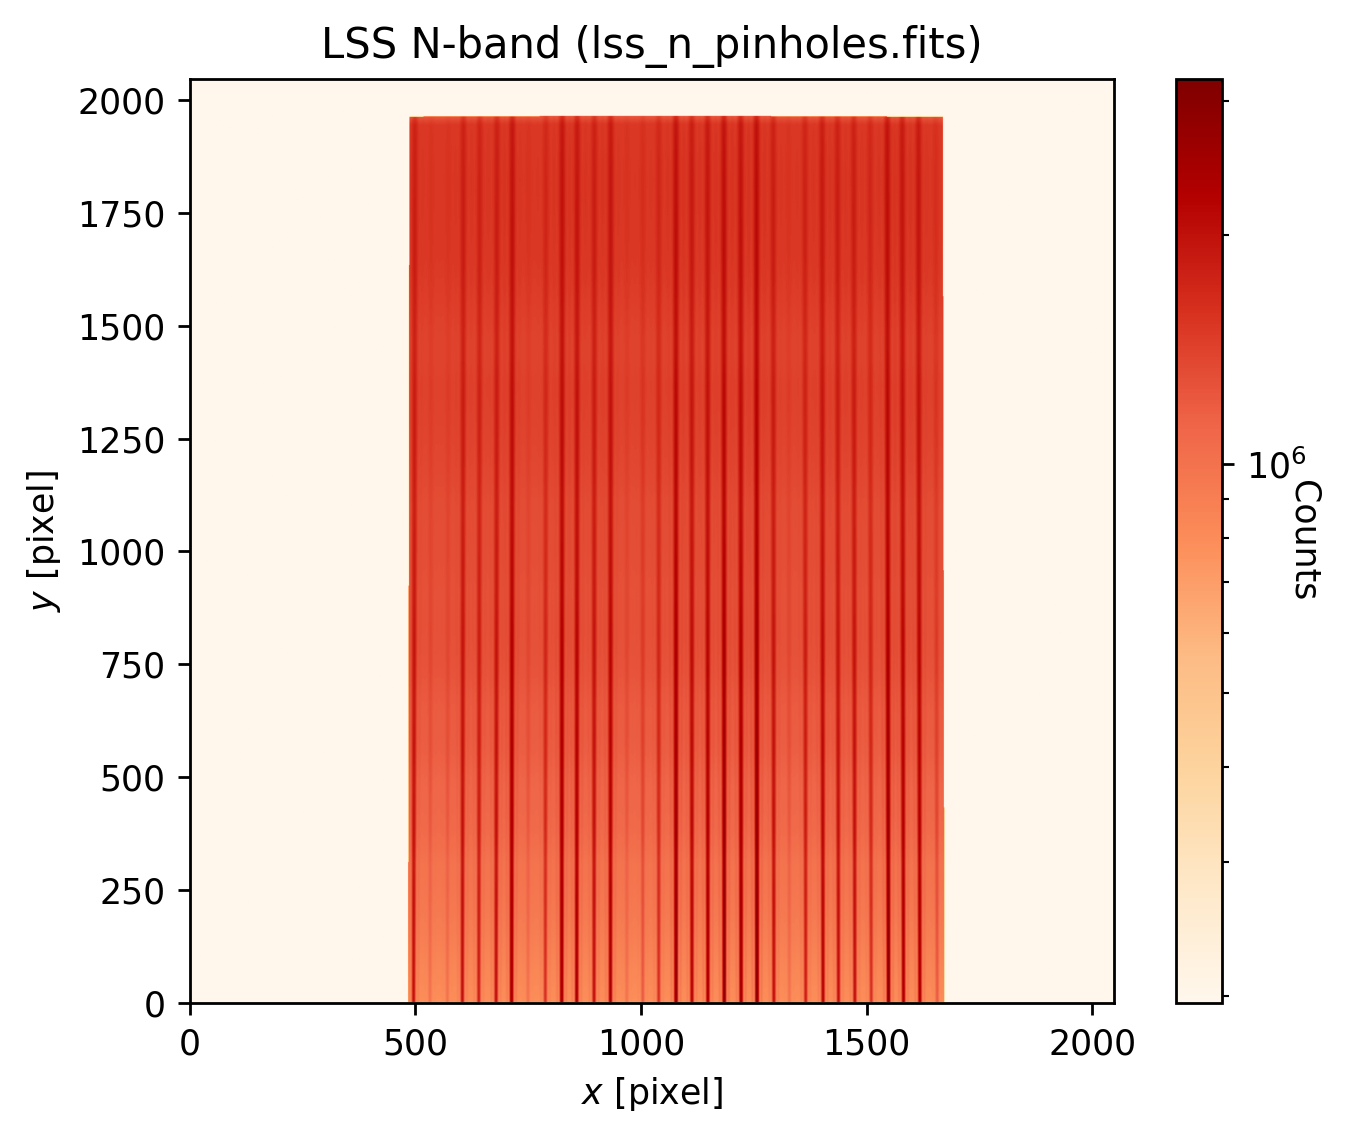
\includegraphics[height=4cm,keepaspectratio]{figures/LSS_CrtAlg_files/lss_n_pinholes.fits.png}
  \caption{Pinholes with the flat field frames for \lss~$L$-, $M$-, and $N$-bands.} 
  \label{fig:pinh}
\end{figure}

\begin{figure}[!ht]
\centering
  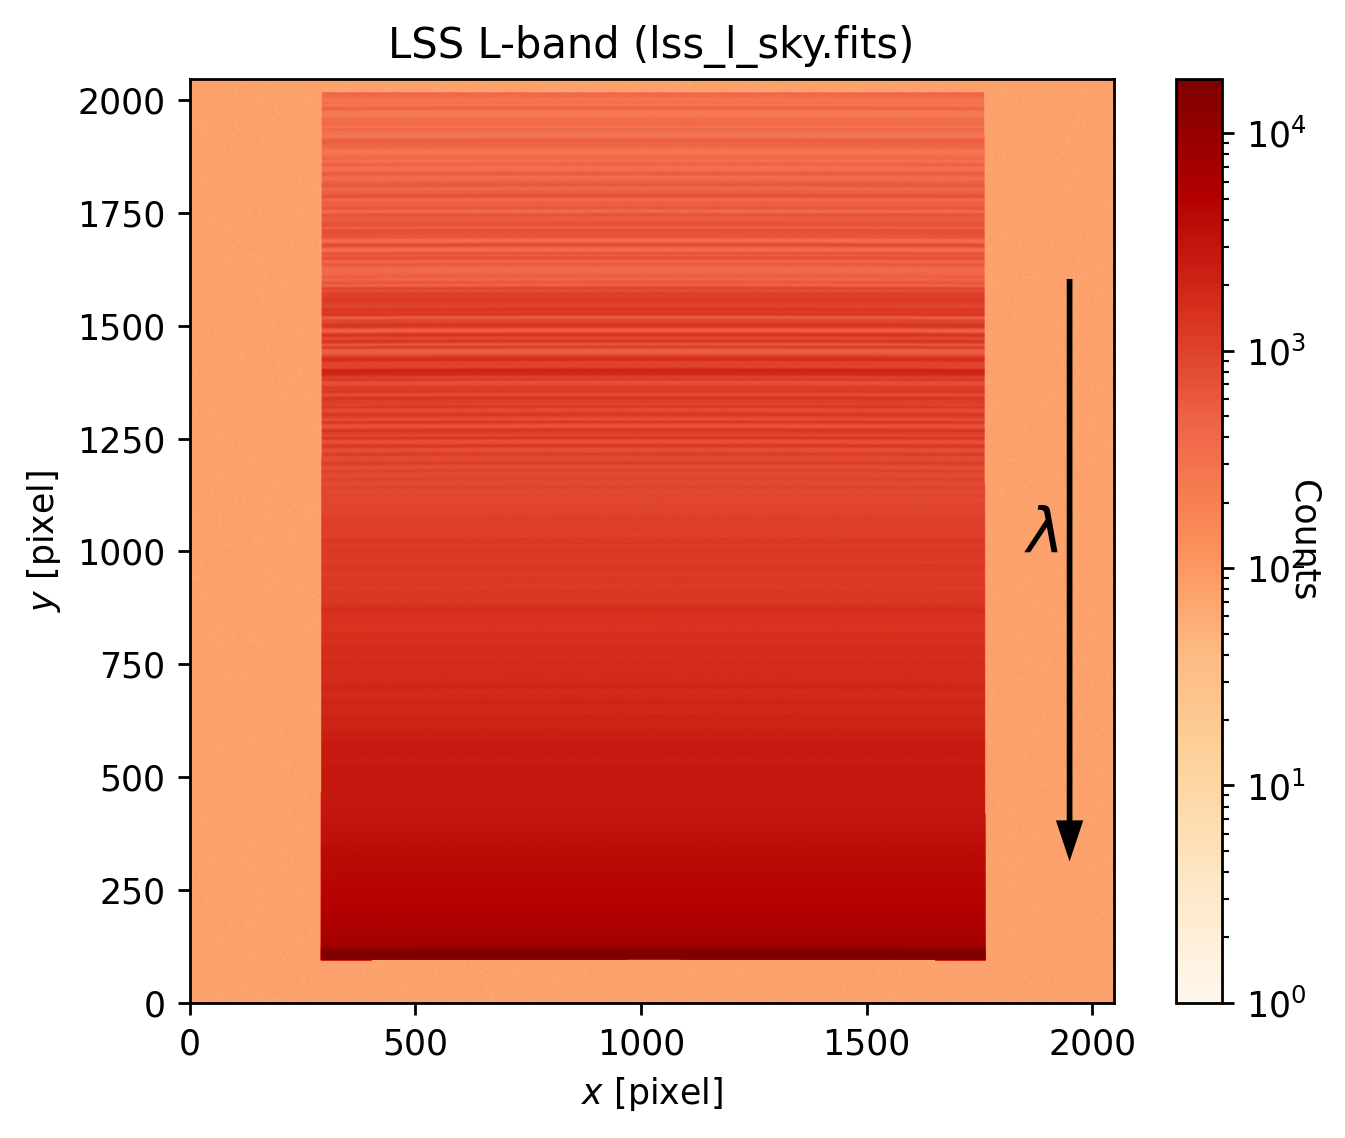
\includegraphics[height=4cm,keepaspectratio]{figures/LSS_CrtAlg_files/lss_l_sky.fits.png}
  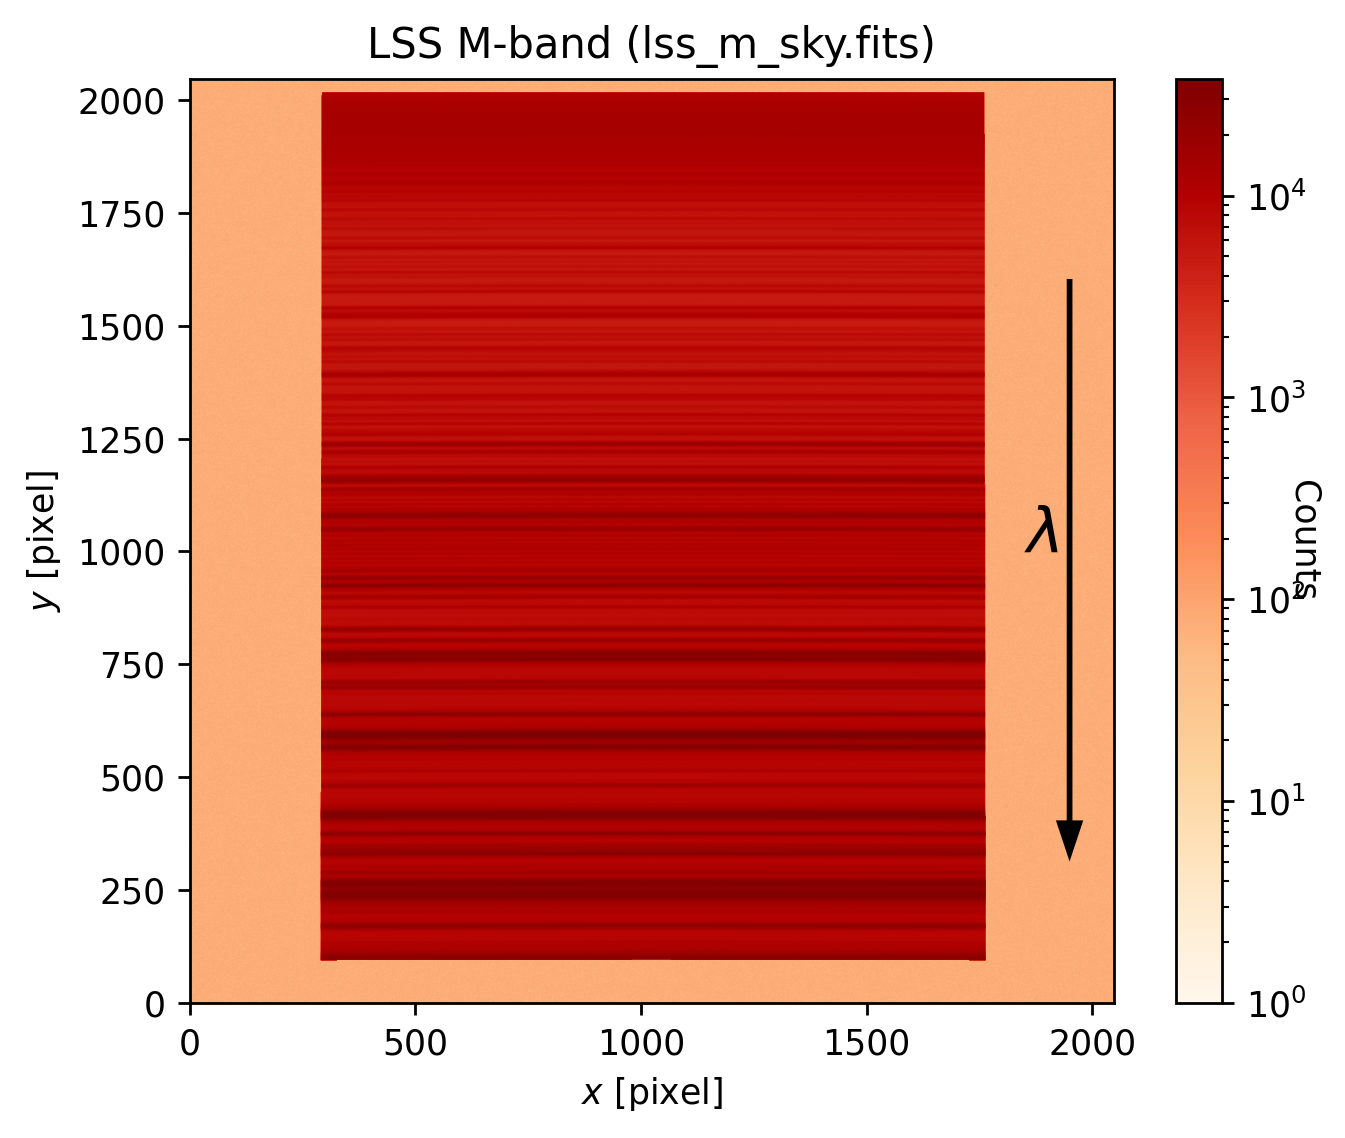
\includegraphics[height=4cm,keepaspectratio]{figures/LSS_CrtAlg_files/lss_m_sky.fits.png}
  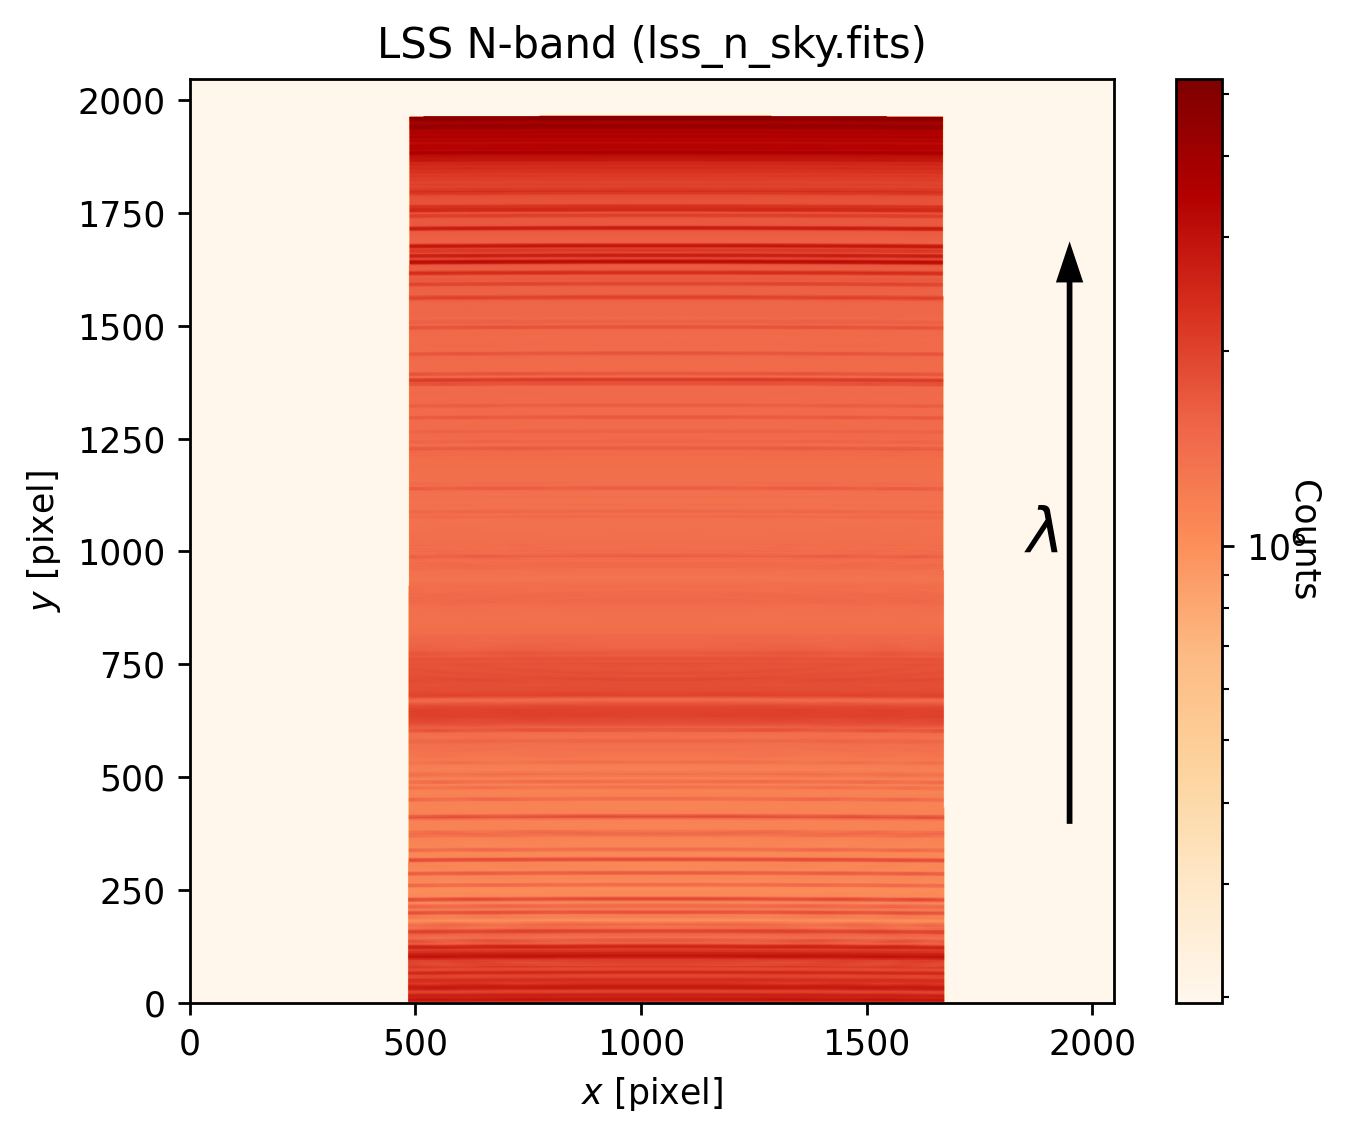
\includegraphics[height=4cm,keepaspectratio]{figures/LSS_CrtAlg_files/lss_n_sky.fits.png}
  \caption{Sky emission line spectrum frames for \lss~$L$-, $M$-, and $N$-bands.} 
  \label{fig:sky}
\end{figure}


\begin{figure}[!ht]
\centering
  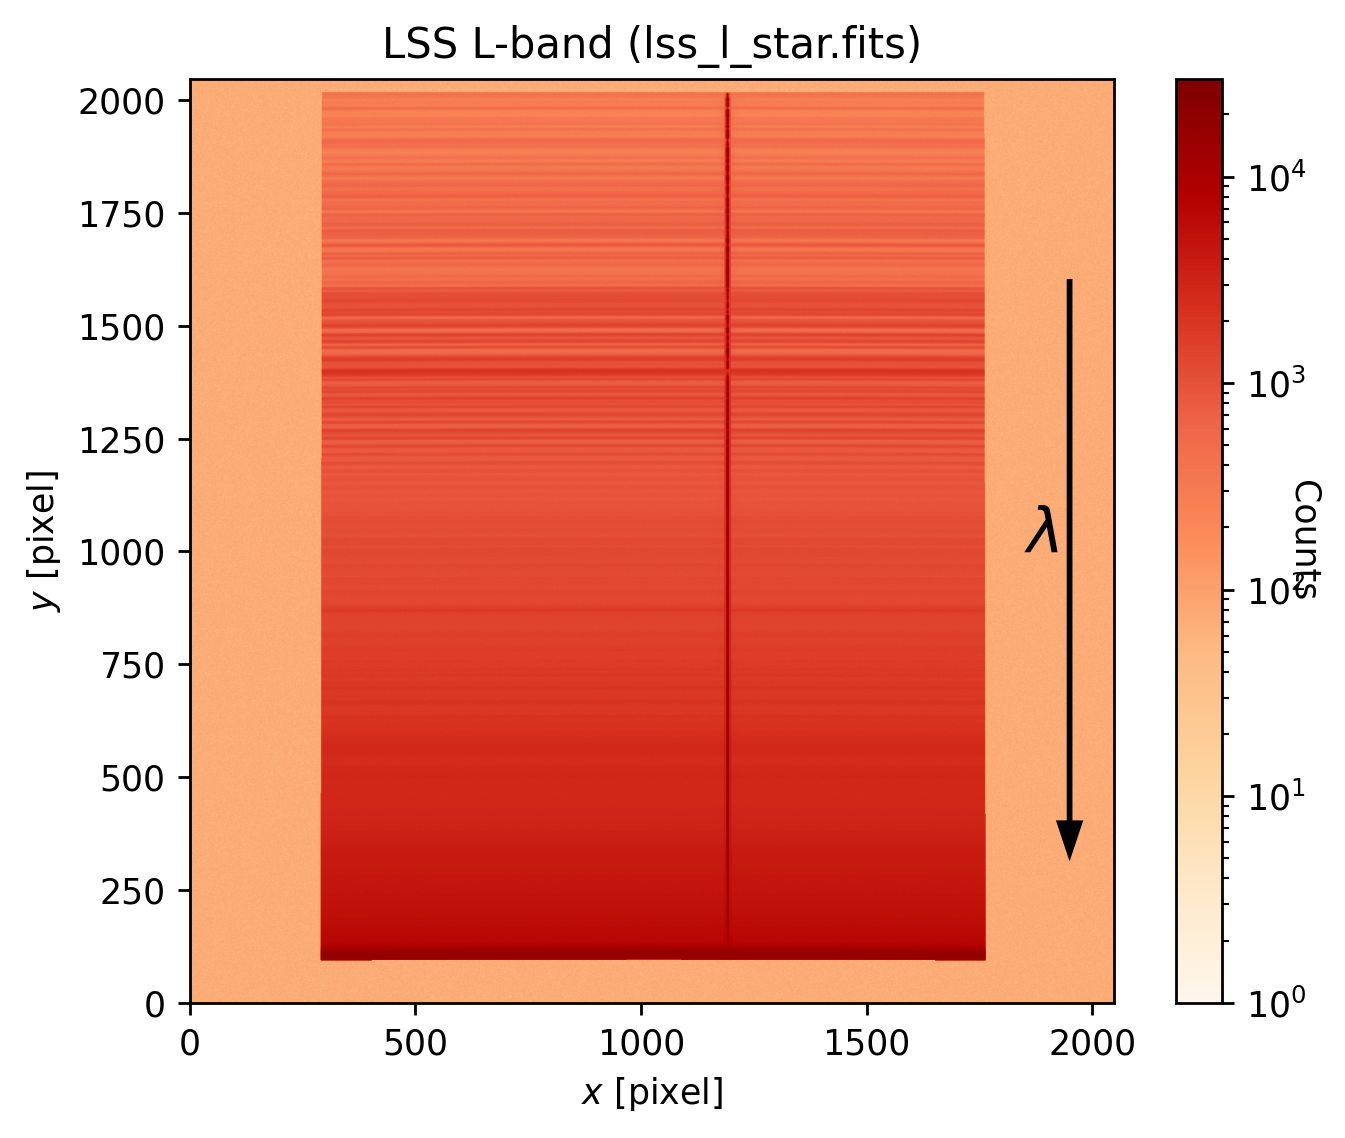
\includegraphics[height=4cm,keepaspectratio]{figures/LSS_CrtAlg_files/lss_l_star.fits.png}
  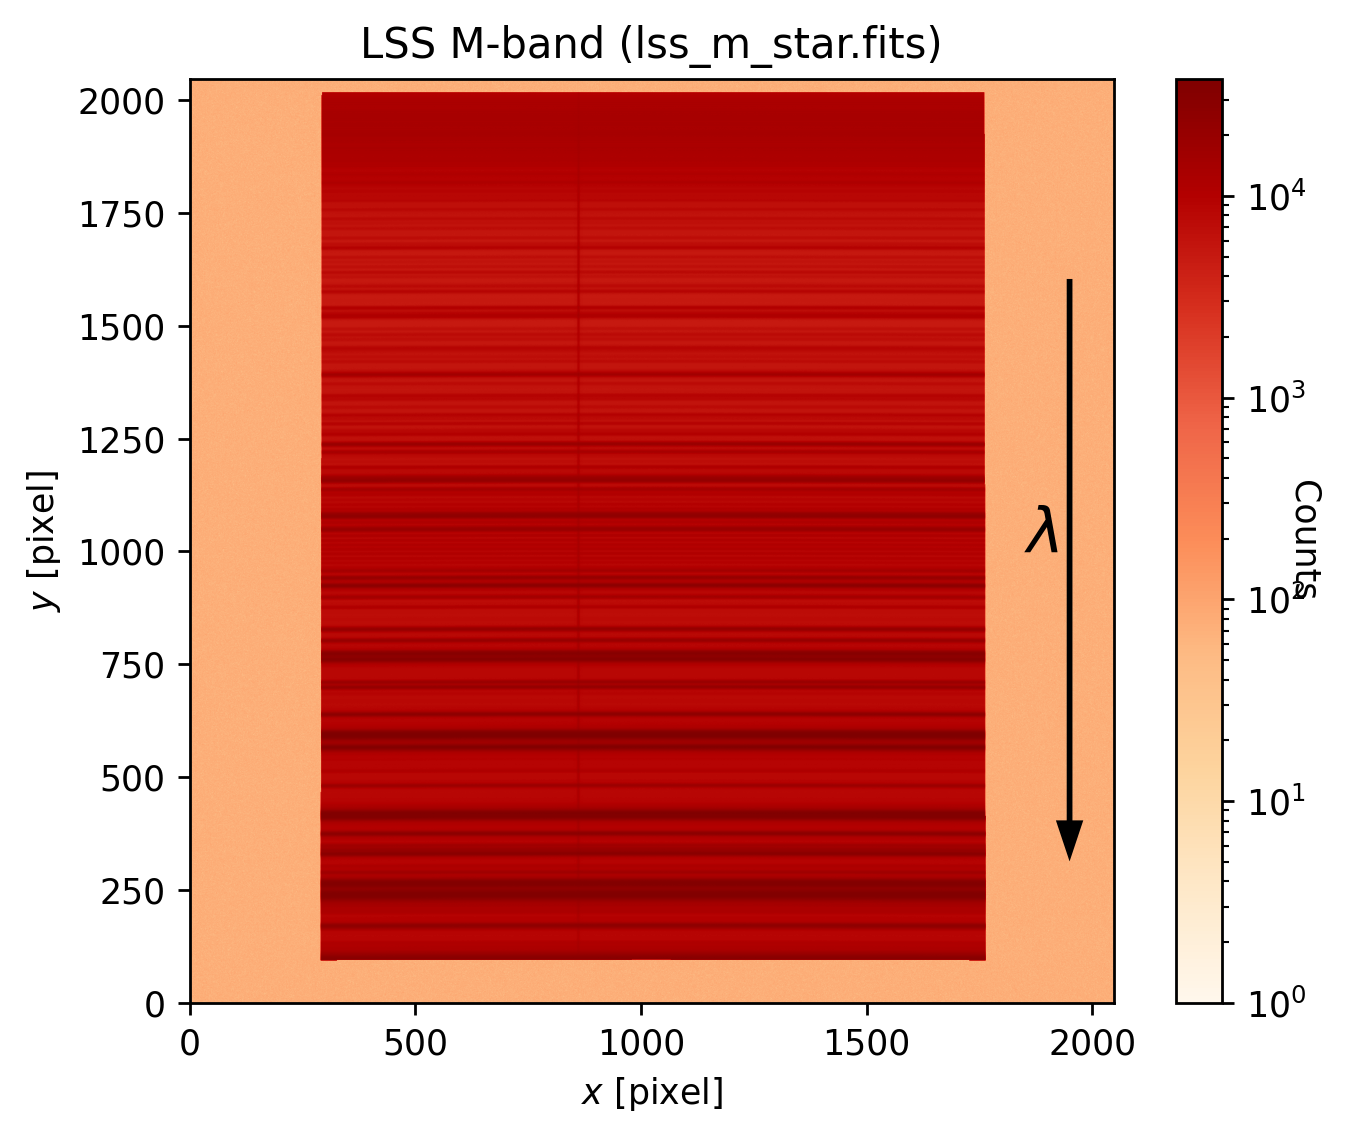
\includegraphics[height=4cm,keepaspectratio]{figures/LSS_CrtAlg_files/lss_m_star.fits.png}
  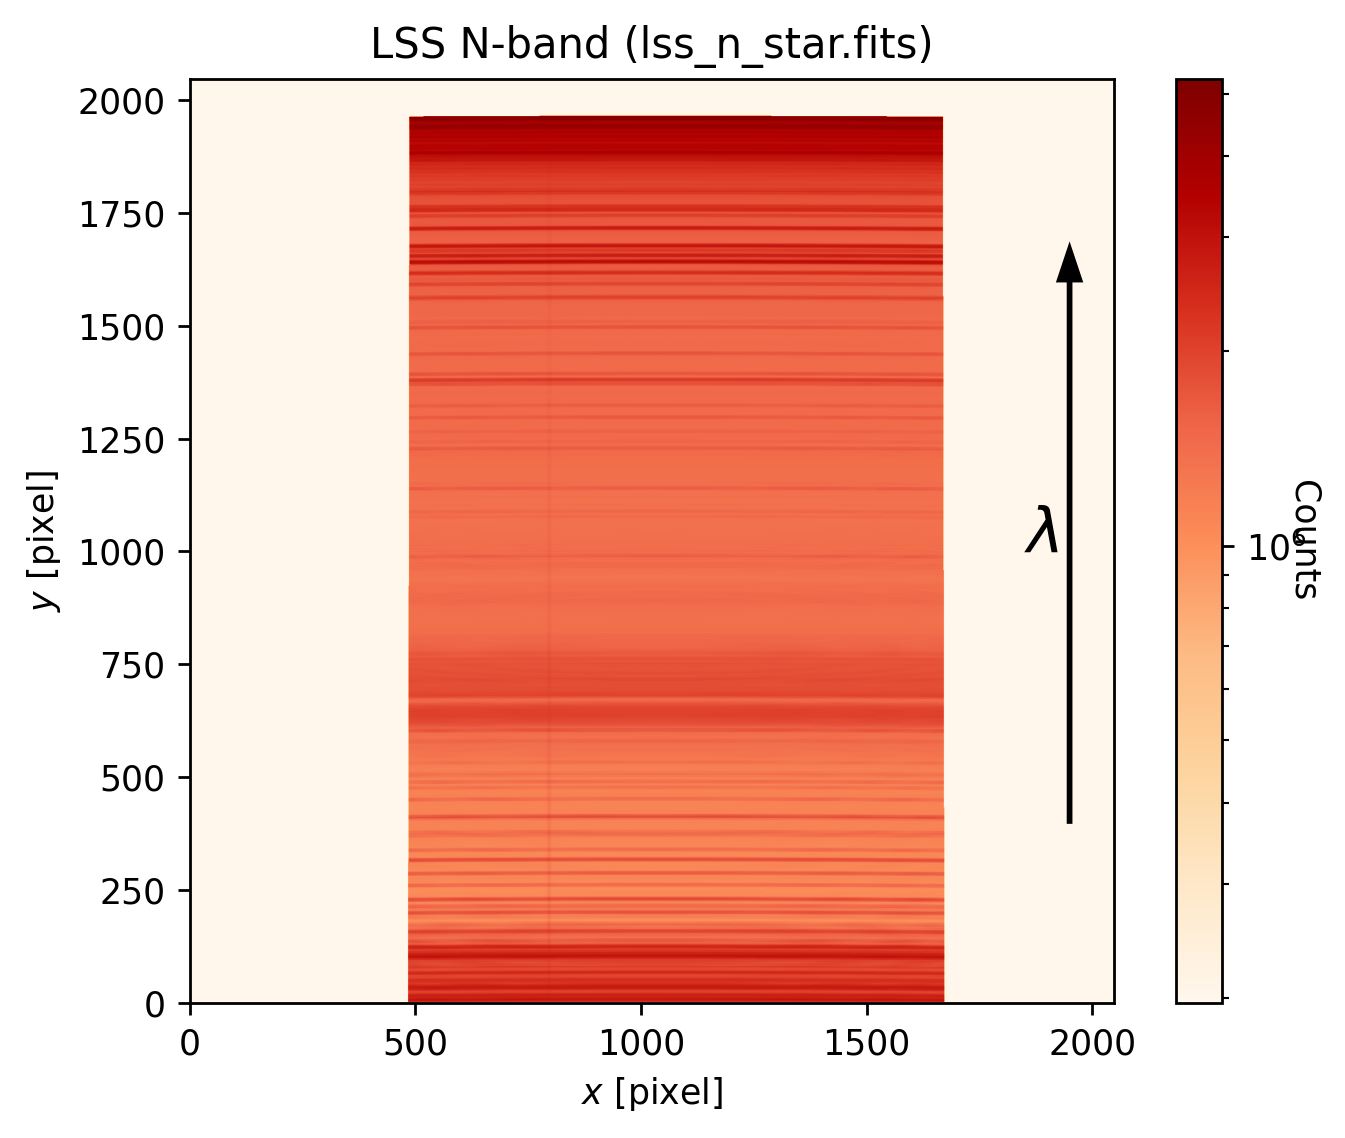
\includegraphics[height=4cm,keepaspectratio]{figures/LSS_CrtAlg_files/lss_n_star.fits.png}
  \caption{Star spectrum ("science" target) frames for \lss~$L$-, $M$-, and $N$-bands.} 
  \label{fig:star}
\end{figure}

%-----------
\paragraph{Installing and running \pyred}\label{sec:pryred_install}

For the purpose of this report, we set up a git repository of a version of \pyred~adapted to work on simulated \met~data. This package can be downloaded from \url{https://github.com/nadsabha/PyReduce_ELT} or installed via Python~3 pip command: \\
\texttt{pip install git+https://github.com/nadsabha/PyReduce\_ELT} \\
The package includes a README file with instructions pertaining to running \pyred~on \elt~data and links to the needed input data (\texttt{README.md})).
% To display the feasibility of adopting \pyred~algorithms The package is so far adapted to work on one detector in the IJ-band short slit. Adaptations  which is 


%-----------
\paragraph{Order detection}\label{sec:critalg_orderdet}
%\todo[inline]{DONE-NS-210730: include report}

\begin{figure}[!ht]
  \centering
  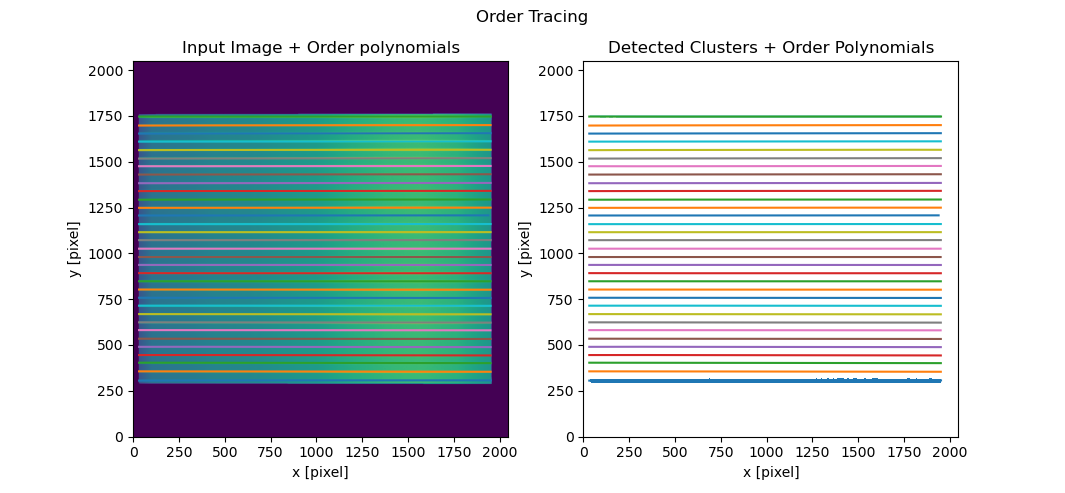
\includegraphics[width=\textwidth]{figures/LSS_CrtAlg_files/Figure_4.png}
  \caption{\textbf{\pyred~output}: Slit traces. Left panel: The fitted order polynomials overlaid on the image of the spectroscopic flat field with the pinholes. Right: The fitted order polynomials overlaid on the detected clusters for the order traces. For \met data, only the central polynomial trace for each trace is returned and used in the subsequent steps. Shown here for the case of \lss~$M$-band. }
  \label{fig:fig3}
\end{figure}

The details of how \pyred~handles the detection of the spectroscopic orders is described in Sect.~\ref{ssec:orderhandling} and \cite{pis02, pis21}. 
\pyred~rotates the images by 90 degrees counter clockwise to align the wavelength dispersion direction along the x-axis and performs the order detection on the pinhole frame with the flat field lamp.  Clusters of neighboring pixels belonging to an order trace are identified  and merged together according to predefined criteria. In the case of \met, a total of thirty three polynomials are fitted as order traces for each slit trace on the detector. These correspond to the pinhole positions of the flat field frame, see Fig.~\ref{fig:fig3}. To correctly extract the trace, the main routine \texttt{reduce.py} is modified to return only the central polynomial fit of each trace on the detector, i.e. fit number 17 (or 16 as per Python convention counted from bottom to up). This allowed a correct extraction of the traces in preparation for the curvature determination step. The order trace fits are stored in the \pyred~output file \texttt{metis\_lss\_m.ord\_default.npz} under \texttt{orders} and \texttt{column\_range} recarrays.
%-----------
\paragraph{Slit curvature}\label{sec:critalg_orderrect}
%\todo[inline]{DONE-NS-210730: include report}

\begin{figure}
\centering
  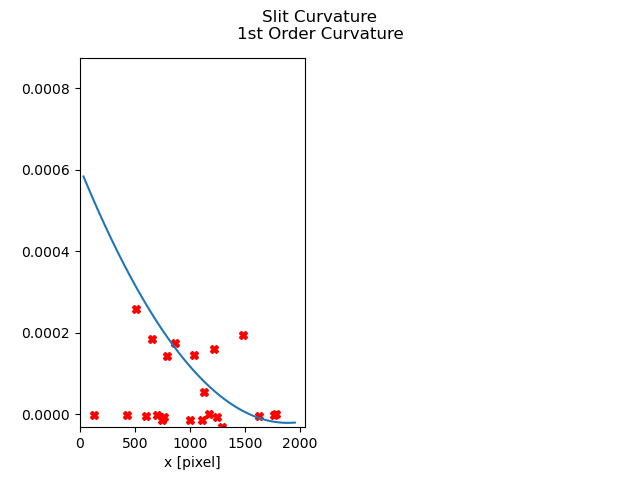
\includegraphics[width=\linewidth]{figures/LSS_CrtAlg_files/Figure_8.png}
  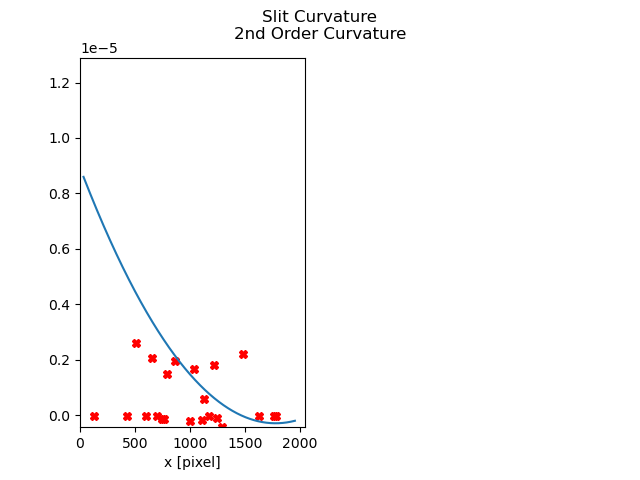
\includegraphics[width=\linewidth]{figures/LSS_CrtAlg_files/Figure_9.png}
  \caption{\textbf{\pyred~output}: Slit curvature tilt (1st order curvature) and shear (2nd order curvature) determination. Shown here for the case of \lss~$M$-band. } 
  \label{fig:fig6n7}
\end{figure}

\pyred~determines the slit curvature by identifying wavelength calibration spectral lines in the extracted order trace and fits the tilt and shear of each order along the image (1st order curvature and 2nd order curvature, respectively). More details on how the package handles slit curvature is discussed in Sect.~\ref{ssec:orderhandling} and \cite{pis21}. 

Figure~\ref{fig:fig6n7} shows the result of the polynomial fitting of the tilt and shear for the extracted slit trace of the \lss~$M$-band file \texttt{lss\_m\_sky.fits}. Figure~\ref{fig:fig8} shows the spectral lines used for the curvature determination  overlaid by the extracted tilt and shear marked in red lines. The x-axis corresponds to the y-axis on the original fits images (Fig~\ref{fig:sky}), while the y-axis of Fig.~\ref{fig:fig8} refers to the order trace number on the detector as \pyred~extracted it. Order~0 is the slit trace of the long slit. The order curvature polynomial fits are stored in the \pyred~output file \texttt{metis\_lss\_m.shear.npz} under \texttt{tilt} and \texttt{shear} recarrays.
\begin{figure}[!ht]
  \centering
  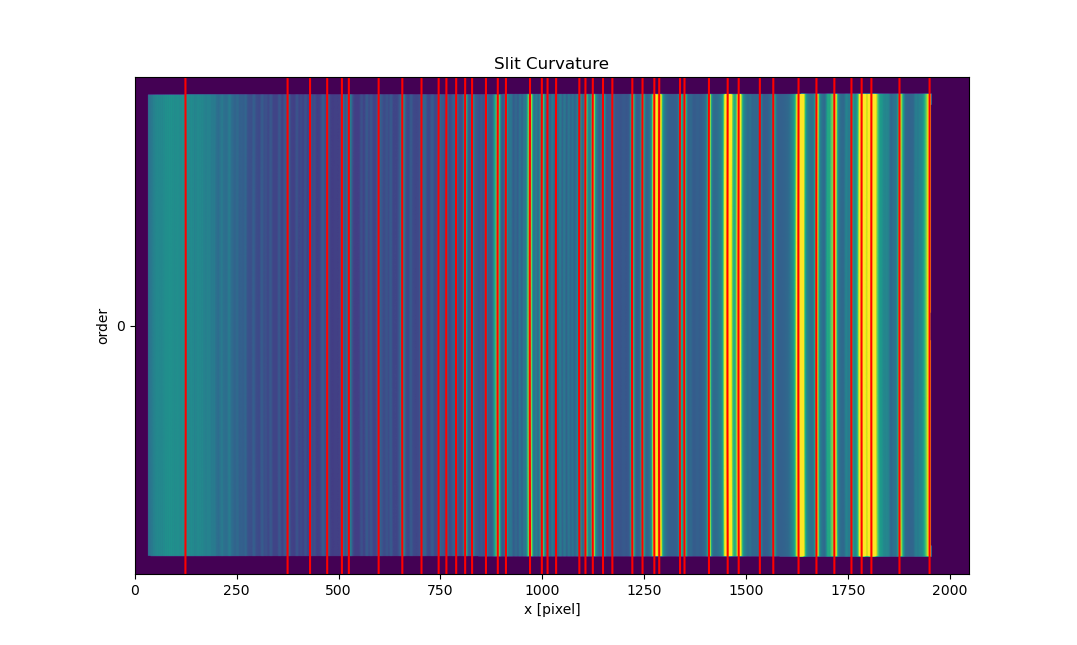
\includegraphics[width=\textwidth]{figures/LSS_CrtAlg_files/Figure_10.png}
  \caption{\textbf{\pyred~output}: Slit curvature determination. The spectral lines used for the curvature determination are overlaid by the extracted tilt and shear fits marked in red lines. Shown here for the case of \lss~$M$-band.}
  \label{fig:fig8}
\end{figure}

%-----------
\paragraph{Wavelength calibration}\label{sec:critalg_wavecal}
%\todo[inline]{DONE-NS-210730: include report}

The algorithm for the wavelength calibration strategy is described in Sect.~\ref{ssec:wavecal} and in \cite{pis02, pis21}. Here we describe and assess the performance of \pyred. 




\begin{figure}[!ht]
  \centering
  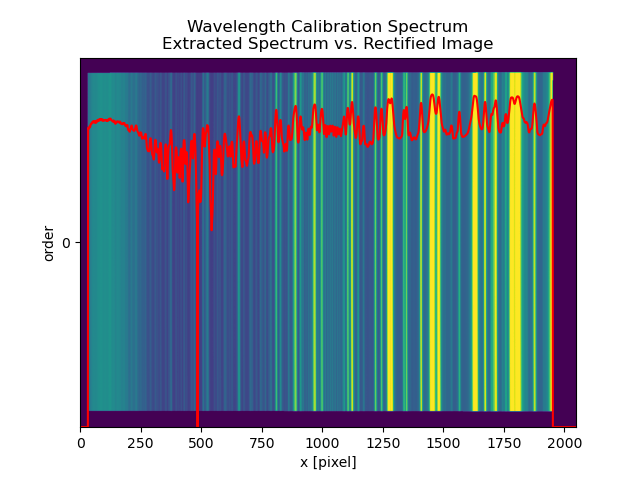
\includegraphics[width=\textwidth]{figures/LSS_CrtAlg_files/Figure_12.png}
  \caption{\textbf{\pyred~output}: Wavelength calibration extracted spectrum. Shown here for the case of \lss~$M$-band.}
  \label{fig:fig9}
\end{figure}

After the order tracing, extraction and curvature (tilt and shear) determination, \pyred~extracts can proceed with extracting a wavelength calibration spectrum for each order (here only one since we have an \lss~mode) from the wavelength calibration frame (\texttt{lss\_m\_sky.fits}, Fig.~\ref{fig:fig9}). The order spectrum is then compared to the wavelength calibration guess file \texttt{metis\_lss\_m\_2D.npz} of the \lss~$M$-band.  The \texttt{npz} file includes a numpy recarray called \texttt{cs\_lines} which lists mainly the wavelengths of the calibration reference lines, the x-pixel positions for start, center, and the end of each of the line traces on the detector, and the corresponding order as per \pyred~detection convention (here is zero in the case of \met~\lss). The list of reference lines and their positions on the detector was obtained by cross-matching their wavelengths  with the spectral layout of \met~\lss~for each band as obtained from the \met~IRDB\footnote{Instrument Reference Database, \url{https://github.com/AstarVienna/irdb/tree/dev_master/METIS}} and implemented in \scope~(e.g. \texttt{TRACE\_LSS\_M.fits}, see also Figure~\ref{fig:lmn_layout}). \pyred~then performs a cross-correlation to determine any offset between the reference (green lines) and the observation (red lines) as shown in \pyred~intermediate output file in Fig.~\ref{fig:fig10}.
\begin{figure}[!ht]
  \centering
  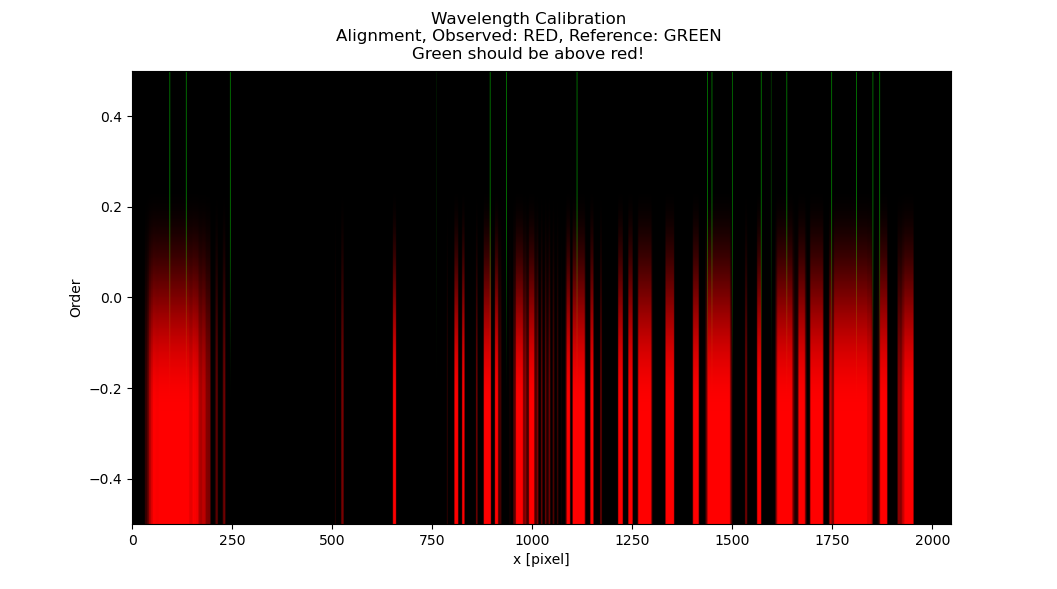
\includegraphics[width=\textwidth]{figures/LSS_CrtAlg_files/Figure_13.png}
  \caption{\textbf{\pyred~output}: Lines used for the wavelength calibration. The reference lines (green) and the observed lines (red) are aligned to each other for each order, where the green reference lines are shown to the top of the red observed line.  Shown here for the case of \lss~$M$-band.}
  \label{fig:fig10}
\end{figure}

Wavelength calibration residuals are then calculated for matching lines and a wavelength solution  is found. The wavelength solution for \met~\lss~is found by fitting a 2D polynomial, with degrees of 4 and 4 in the dispersion and the spatial direction, respectively. Figure~\ref{fig:fig12} bottom panel shows the 2D wavelength solution of the extracted slit trace where it can be seen that the wavelength range and increment of the trace match the spectral layout on detector one as seen in Fig.~\ref{fig:lmn_layout}.  The wavelength calibration spectrum is shown in the top panel of Fig.~\ref{fig:fig12}. The wavelength calibration spectrum is stored in the \pyred~output file \texttt{metis\_lss\_m.thar\_master.fits} and the corresponding wavelength solution in \texttt{metis\_lss\_m.thar.npz} recarrays \texttt{wave} and \texttt{coef}, while a modified list of the wavelength calibration lines is returned  in \texttt{linelist} indicating which line was used in the fitting procedure. 

\begin{figure}[!ht]
  \centering
  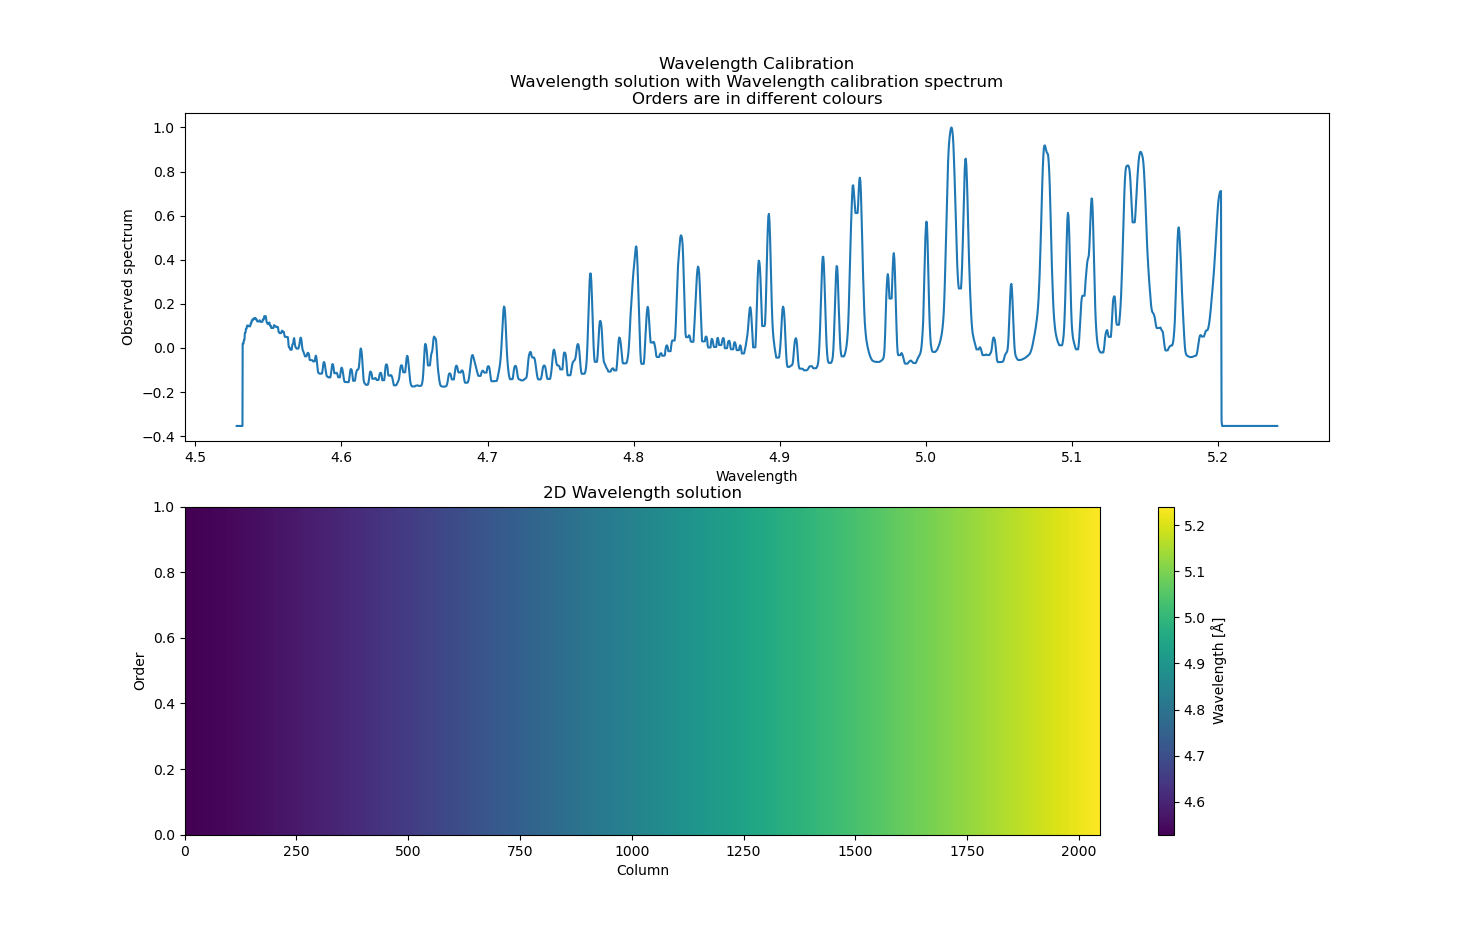
\includegraphics[width=\textwidth]{figures/LSS_CrtAlg_files/Figure_15.png}
  \caption{\textbf{\pyred~output}: Top: Wavelength calibration spectrum for  \lss~$M$-band. Bottom: 2D wavelength solution of \pyred~order~0 (\lss slit trace). The x-axis (Column) refers to the y pixel of the detector image in Fig.~\ref{fig:lmn_layout}. }
  \label{fig:fig12}
\end{figure}



% HB 20230630: I commented this out because fig:r_m is also commented out.
% To assess the accuracy of the wavelength solution, the extracted wavelength calibration spectrum is compared to the input sky spectrum \texttt{SKYCALC\_LSS\_override.fits} from \met~IRDB (see Figure~\ref{fig:sky_spec}). The sky spectrum is based on \textsc{Skycalc}, which is in turn based on \textsc{HITRAN}\footnote{\url{www.hitran.org}}. Figure~\ref{fig:r_m} top panel show the spectrum extracted by \pyred. The vertical dashed lines indicate the reference wavelength of each detected calibration sky line. The bottom panel shows the residuals between the reference wavelength and fitted wavelength (line center) of each detected calibration line divided by its $FWHM$. As can be seen, the calculated residuals are within $\pm 0.1 \times~FWHM$ for most lines.

\begin{figure}[!ht]
  \centering
  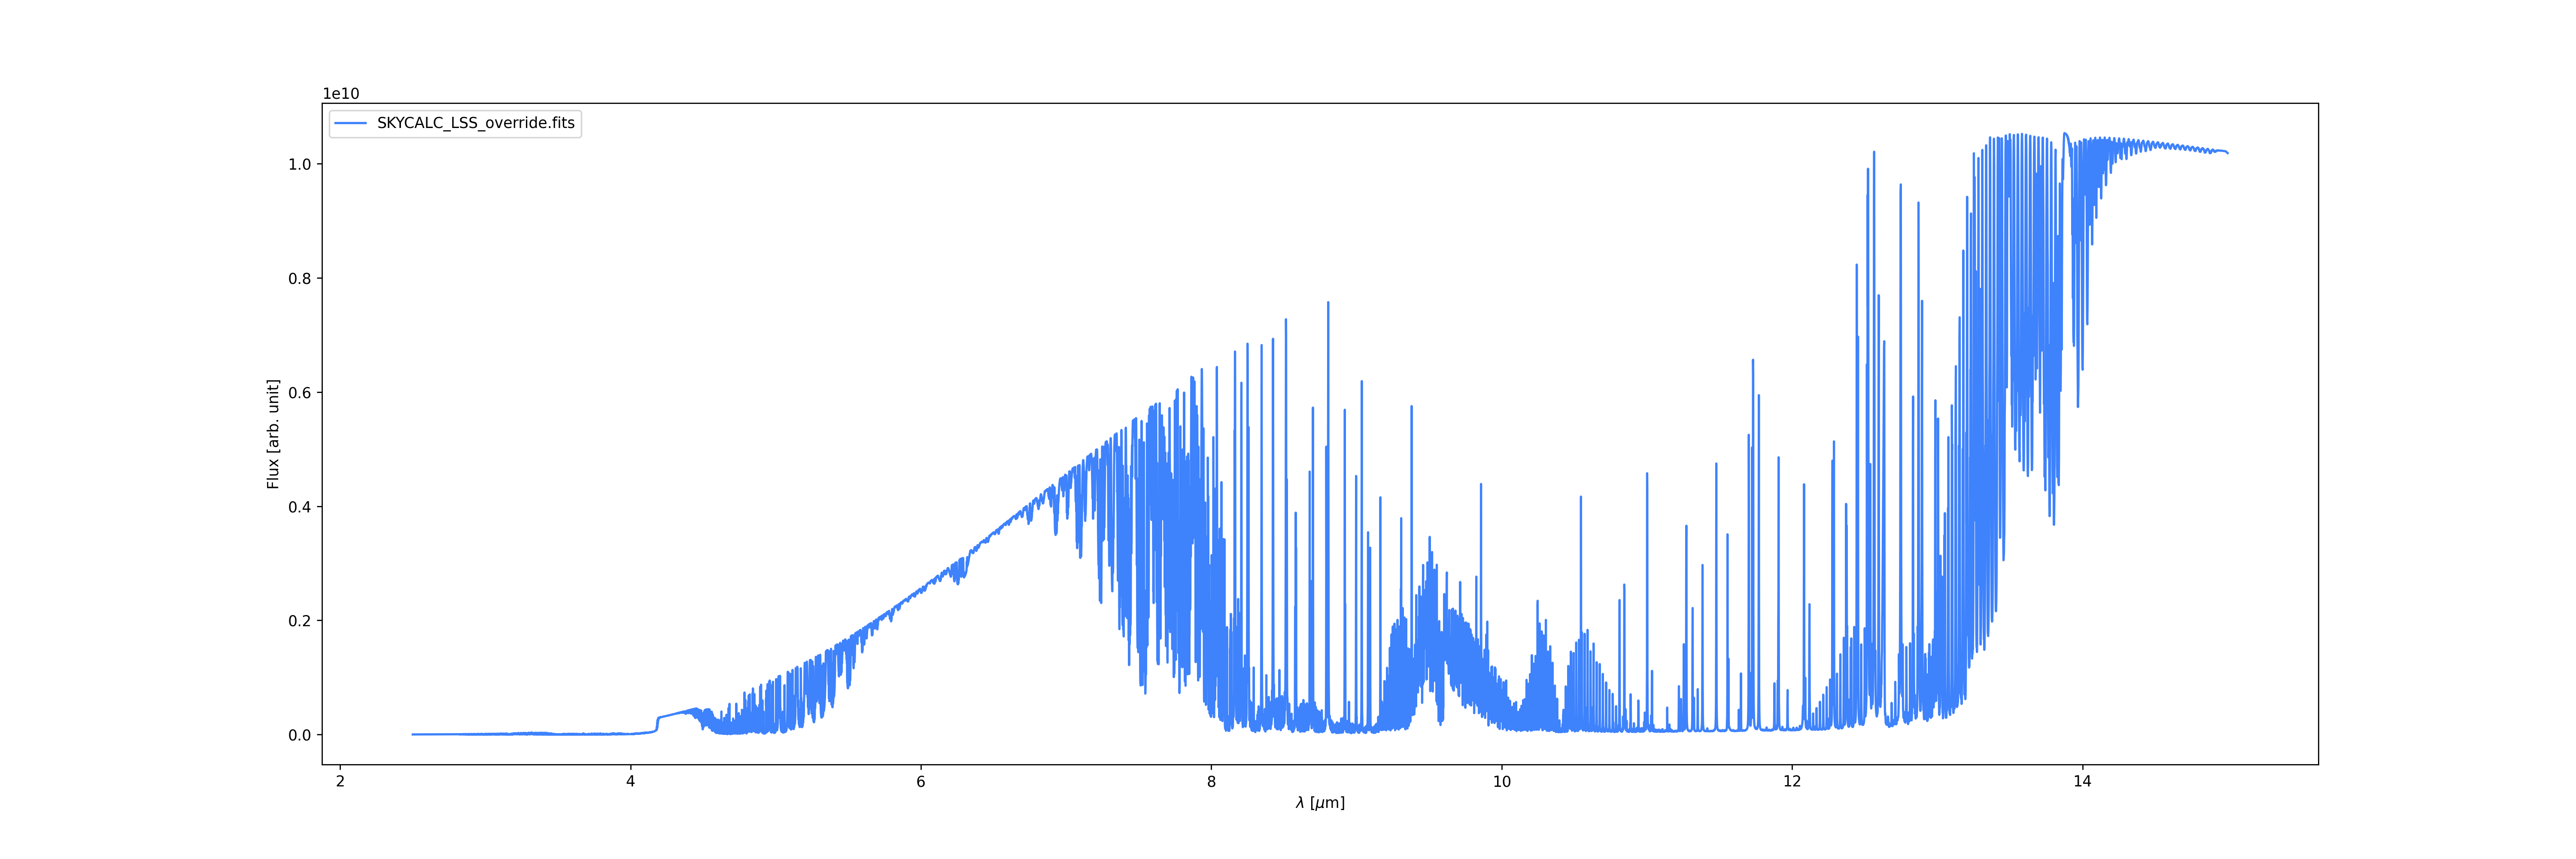
\includegraphics[width=\textwidth]{figures/LSS_CrtAlg_files/SKYCALC_LSS_override.fits.png}
  \caption{\textbf{Input sky spectrum over the wavelength range covered by \met~\lss modes}: The sky spectrum is taken from \met~IRDB file \texttt{SKYCALC\_LSS\_override.fits}. }
  \label{fig:sky_spec}
\end{figure}

% \subparagraph{Wavelength calibration accuracy}\label{sec:critalg_wavecal_acc}
% \begin{figure}[!ht]
%   \centering
%   \includegraphics[width=0.8\textwidth]{figures/LSS_CrtAlg_files/Residuals_72.png}
%   \caption{Residuals of the wavelength calibration for \lss~$M$-band. The top panel displays the extracted wavelength calibration spectrum. The bottom panel shows the residuals of the wavelength calibration divided by the $FWHM$ of each respective line. The vertical dotted lines are the reference wavelengths of the input sky emission lines. }
%   \label{fig:r_m}
% \end{figure}

% \begin{figure}[!ht]
%   \centering
%   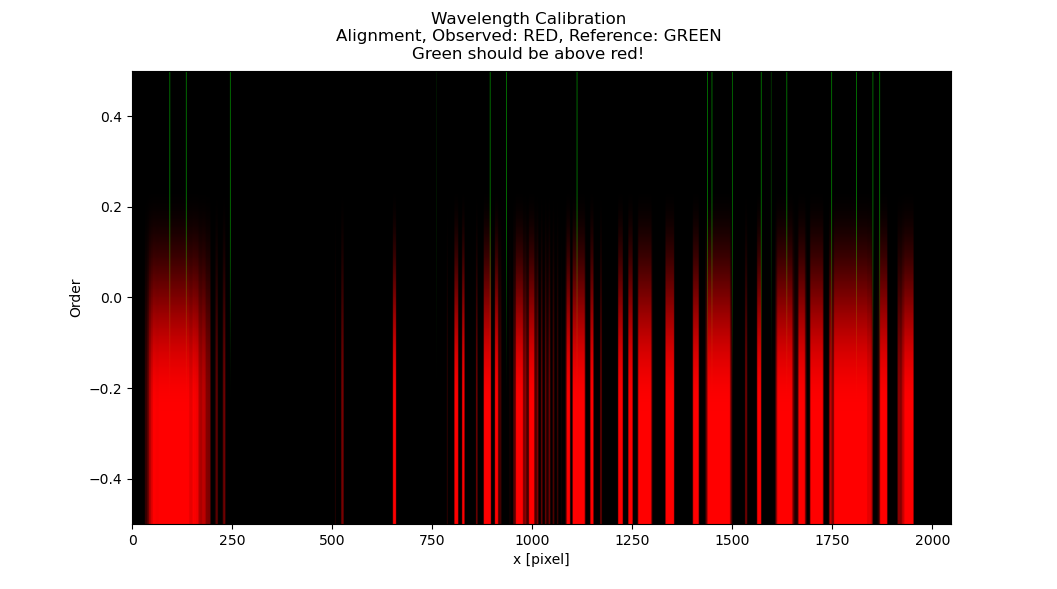
\includegraphics[width=\textwidth]{figures/LSS_CrtAlg_files/Figure_13.png}
%   \caption{\textbf{\pyred~output}: Extracted spectrum from a simulated science frame overlaid on the rectified order images. }
%   \label{fig:fig13}
% \end{figure}

% Figure~\ref{fig:fig13} shows the extracted and rectified spectrum from the frame \texttt{IJ\_freqcomb\_newheaders.fits} (Fig.~\ref{fig:star}) where an optimal extraction is performed using the \pyred~step \texttt{"science"}. 

\paragraph{Summary}
We showed  that the \pyred~package (currently part of CRIRES+ pipeline) can be adapted to work on simulated \met~\lss~data in all bands by creating the needed \pyred~files and tweaking the parameters used for each of the reduction steps (see linked package). All three steps of order detection, curvature determination, and wavelength calibration are successfully implemented. Further tweaking of certain parameters may be needed to improve the individual steps.


% The current setup of \pyred~assumes that each detector is to be treated individually, therefore we focused on adapting  it to the first detector of the IJ-band short slit. For a full implementation, we will create wavelength calibration guess files  for the remaining detectors, bands, and slits, to be treated in similar fashion to what we just showed. Alternatively for future prospects, one could consider combining all nine detectors into one large image by updating the instrument class and alternating one of the core routines of \pyred~that first reads the data and prepares it for the analysis (private communication with Ansgar Wehrhahn). 


